% ════════════════════════════════════════════
% 6. 模型建立与结果分析
% ════════════════════════════════════════════
\section{模型建立与结果分析}

\subsection{模型设定与候选比较}

因变量取 $\log(1+Y_1)$，解释变量为发帖决策变量与时间控制项，估计方法为普通最小二乘、推断采用 HC3 稳健标准误。设定从“全模型”出发逐步剔除不可识别或冗余的项，形成五个候选：M0 为均值基线，M1 为含粉丝规模与月份的全模型，M2 去掉粉丝规模、保留月份固定效应，M3 只留粉丝规模，M4 用线性月份替代月份哑变量。五个候选的拟合与十折交叉验证结果见表\ref{tab:cv}：M2 的交叉验证 $R^2$ 最高（0.101）、CV RMSE 最低（1.101），样本内 $R^2=0.207$、调整 $R^2=0.165$；M1 多一个参数而交叉验证表现反而略差，说明粉丝规模提供的是与月份重复的信息。M0 的交叉验证 $R^2$ 为 $-0.021$，均值基线不具备预测能力。

{\small
\begin{longtable}{>{\centering\arraybackslash}p{0.080\textwidth}>{\centering\arraybackslash}p{0.100\textwidth}>{\centering\arraybackslash}p{0.090\textwidth}>{\centering\arraybackslash}p{0.105\textwidth}>{\centering\arraybackslash}p{0.100\textwidth}>{\centering\arraybackslash}p{0.115\textwidth}>{\centering\arraybackslash}p{0.100\textwidth}>{\centering\arraybackslash}p{0.115\textwidth}>{\centering\arraybackslash}p{0.115\textwidth}}
  \caption{五个候选模型的拟合、整体显著性与十折交叉验证}
  \label{tab:cv} \\
  \toprule
  模型 & 参数个数 & $R^2$ & 调整 $R^2$ & 整体 $F$ & $F$ 检验 $p$ & CV $R^2$ & CV RMSE & CV MAE \\
  \midrule
  \endfirsthead
  \caption{五个候选模型的拟合、整体显著性与十折交叉验证（续）} \\
  \toprule
  模型 & 参数个数 & $R^2$ & 调整 $R^2$ & 整体 $F$ & $F$ 检验 $p$ & CV $R^2$ & CV RMSE & CV MAE \\
  \midrule
  \endhead
  \bottomrule
  \endfoot
  M0 & 1 & 0 & 0 & — & — & -0.0212 & 1.1753 & 0.9133 \\
  M1 & 27 & 0.2069 & 0.1633 & 4.7465 & $<$0.001 & 0.0972 & 1.1031 & 0.8351 \\
  M2 & 26 & 0.2068 & 0.1650 & 4.9443 & $<$0.001 & 0.1010 & 1.1007 & 0.8328 \\
  M3 & 16 & 0.1606 & 0.1346 & 6.1756 & $<$0.001 & 0.0935 & 1.1065 & 0.8220 \\
  M4 & 17 & 0.1664 & 0.1388 & 6.0265 & $<$0.001 & 0.0972 & 1.1042 & 0.8215 \\
\end{longtable}
}


\subsection{估计结果}

最终模型 M2 的系数见表\ref{tab:coef}。控制月份、星期、时段后，付费帖子的 $\log(1+Y_1)$ 比自然帖子高 0.337（HC3 标准误 0.120，$p=0.005$）；类型维度上，Status 与 Video 分别比 Photo 高 1.154 与 1.590，Link 与 Photo 无显著差异（$p=0.643$）；主题 2 与主题 3 分别比主题 1 低 0.478 与 0.315，前者 $p<0.001$、后者 $p=0.019$；凌晨与下午晚间相对上午不显著（$p=0.150$、$p=0.638$），星期各水平同样不显著。模型常数项 9.247 对应基准组合（Photo、主题 1、1 月、周一、上午、自然帖）的期望对数曝光。图\ref{fig:forest}把主效应点估计与 95\% 置信区间并排呈现，显著为正、显著为负与不显著三档分别用深蓝、红与灰区分。

{\small
\begin{longtable}{>{\centering\arraybackslash}p{0.240\textwidth}>{\centering\arraybackslash}p{0.100\textwidth}>{\centering\arraybackslash}p{0.100\textwidth}>{\centering\arraybackslash}p{0.080\textwidth}>{\centering\arraybackslash}p{0.120\textwidth}>{\centering\arraybackslash}p{0.120\textwidth}>{\centering\arraybackslash}p{0.080\textwidth}>{\centering\arraybackslash}p{0.080\textwidth}}
  \caption{最终模型 M2 的系数估计}
  \label{tab:coef} \\
  \toprule
  变量 & 系数 & 标准误 & $p$ & CI 下限 & CI 上限 & VIF & 显著性 \\
  \midrule
  \endfirsthead
  \caption{最终模型 M2 的系数估计（续）} \\
  \toprule
  变量 & 系数 & 标准误 & $p$ & CI 下限 & CI 上限 & VIF & 显著性 \\
  \midrule
  \endhead
  \bottomrule
  \endfoot
  常数项 & 9.2468 & 0.2052 & $<$0.001 & 8.8436 & 9.65 & — & *** \\
  类型：Status & 1.1538 & 0.1235 & $<$0.001 & 0.9110 & 1.3966 & 1.2748 & *** \\
  类型：Link & 0.1215 & 0.2619 & 0.643 & -0.3930 & 0.6361 & 1.1356 &  \\
  类型：Video & 1.5896 & 0.4017 & $<$0.001 & 0.8003 & 2.3789 & 1.0626 & *** \\
  主题：2 & -0.4784 & 0.1352 & $<$0.001 & -0.7440 & -0.2128 & 1.7829 & *** \\
  主题：3 & -0.3147 & 0.1337 & 0.019 & -0.5775 & -0.0519 & 1.527 & * \\
  月份：2月 & 0.8765 & 0.3037 & 0.004 & 0.2798 & 1.4733 & 2.0388 & ** \\
  月份：3月 & -0.0414 & 0.3095 & 0.894 & -0.6495 & 0.5667 & 2.5431 &  \\
  月份：4月 & 0.3808 & 0.1768 & 0.032 & 0.0333 & 0.7283 & 2.835 & * \\
  月份：5月 & 0.1908 & 0.1710 & 0.265 & -0.1453 & 0.5269 & 2.362 &  \\
  月份：6月 & 0.1491 & 0.1850 & 0.421 & -0.2144 & 0.5125 & 2.82 &  \\
  月份：7月 & 0.3131 & 0.1900 & 0.100 & -0.0603 & 0.6866 & 2.9706 &  \\
  月份：8月 & 0.1120 & 0.2484 & 0.652 & -0.3762 & 0.6002 & 2.3062 &  \\
  月份：9月 & -0.1259 & 0.1877 & 0.503 & -0.4947 & 0.2429 & 2.4259 &  \\
  月份：10月 & -0.4711 & 0.2136 & 0.028 & -0.8909 & -0.0514 & 3.232 & * \\
  月份：11月 & 0.0355 & 0.1956 & 0.856 & -0.3489 & 0.4198 & 2.808 &  \\
  月份：12月 & -0.1012 & 0.1644 & 0.538 & -0.4242 & 0.2218 & 2.8513 &  \\
  星期：周二 & 0.0939 & 0.1977 & 0.635 & -0.2946 & 0.4823 & 1.7593 &  \\
  星期：周三 & -0.0191 & 0.1920 & 0.921 & -0.3963 & 0.3582 & 1.7682 &  \\
  星期：周四 & 0.2585 & 0.2084 & 0.215 & -0.1509 & 0.6679 & 1.847 &  \\
  星期：周五 & -0.0929 & 0.1770 & 0.600 & -0.4407 & 0.2548 & 1.7946 &  \\
  星期：周六 & -0.1607 & 0.1852 & 0.386 & -0.5246 & 0.2032 & 1.9324 &  \\
  星期：周日 & -0.2214 & 0.1753 & 0.207 & -0.5658 & 0.1231 & 1.8974 &  \\
  时段：凌晨 & 0.1643 & 0.1139 & 0.150 & -0.0595 & 0.3881 & 1.3177 &  \\
  时段：下午晚间 & 0.0751 & 0.1595 & 0.638 & -0.2383 & 0.3885 & 1.5198 &  \\
  付费（X7=1） & 0.3374 & 0.1195 & 0.005 & 0.1025 & 0.5723 & 1.0772 & ** \\
  \bottomrule
\end{longtable}
}
\vspace{-4pt}
{\footnotesize\raggedright 注：标准误为 HC3 稳健标准误；CI 为 95\% 置信区间；*** 为 $p<0.001$，** 为 $p<0.01$，* 为 $p<0.05$。\par}
\vspace{4pt}


\begin{figure}[htbp]
  \centering
  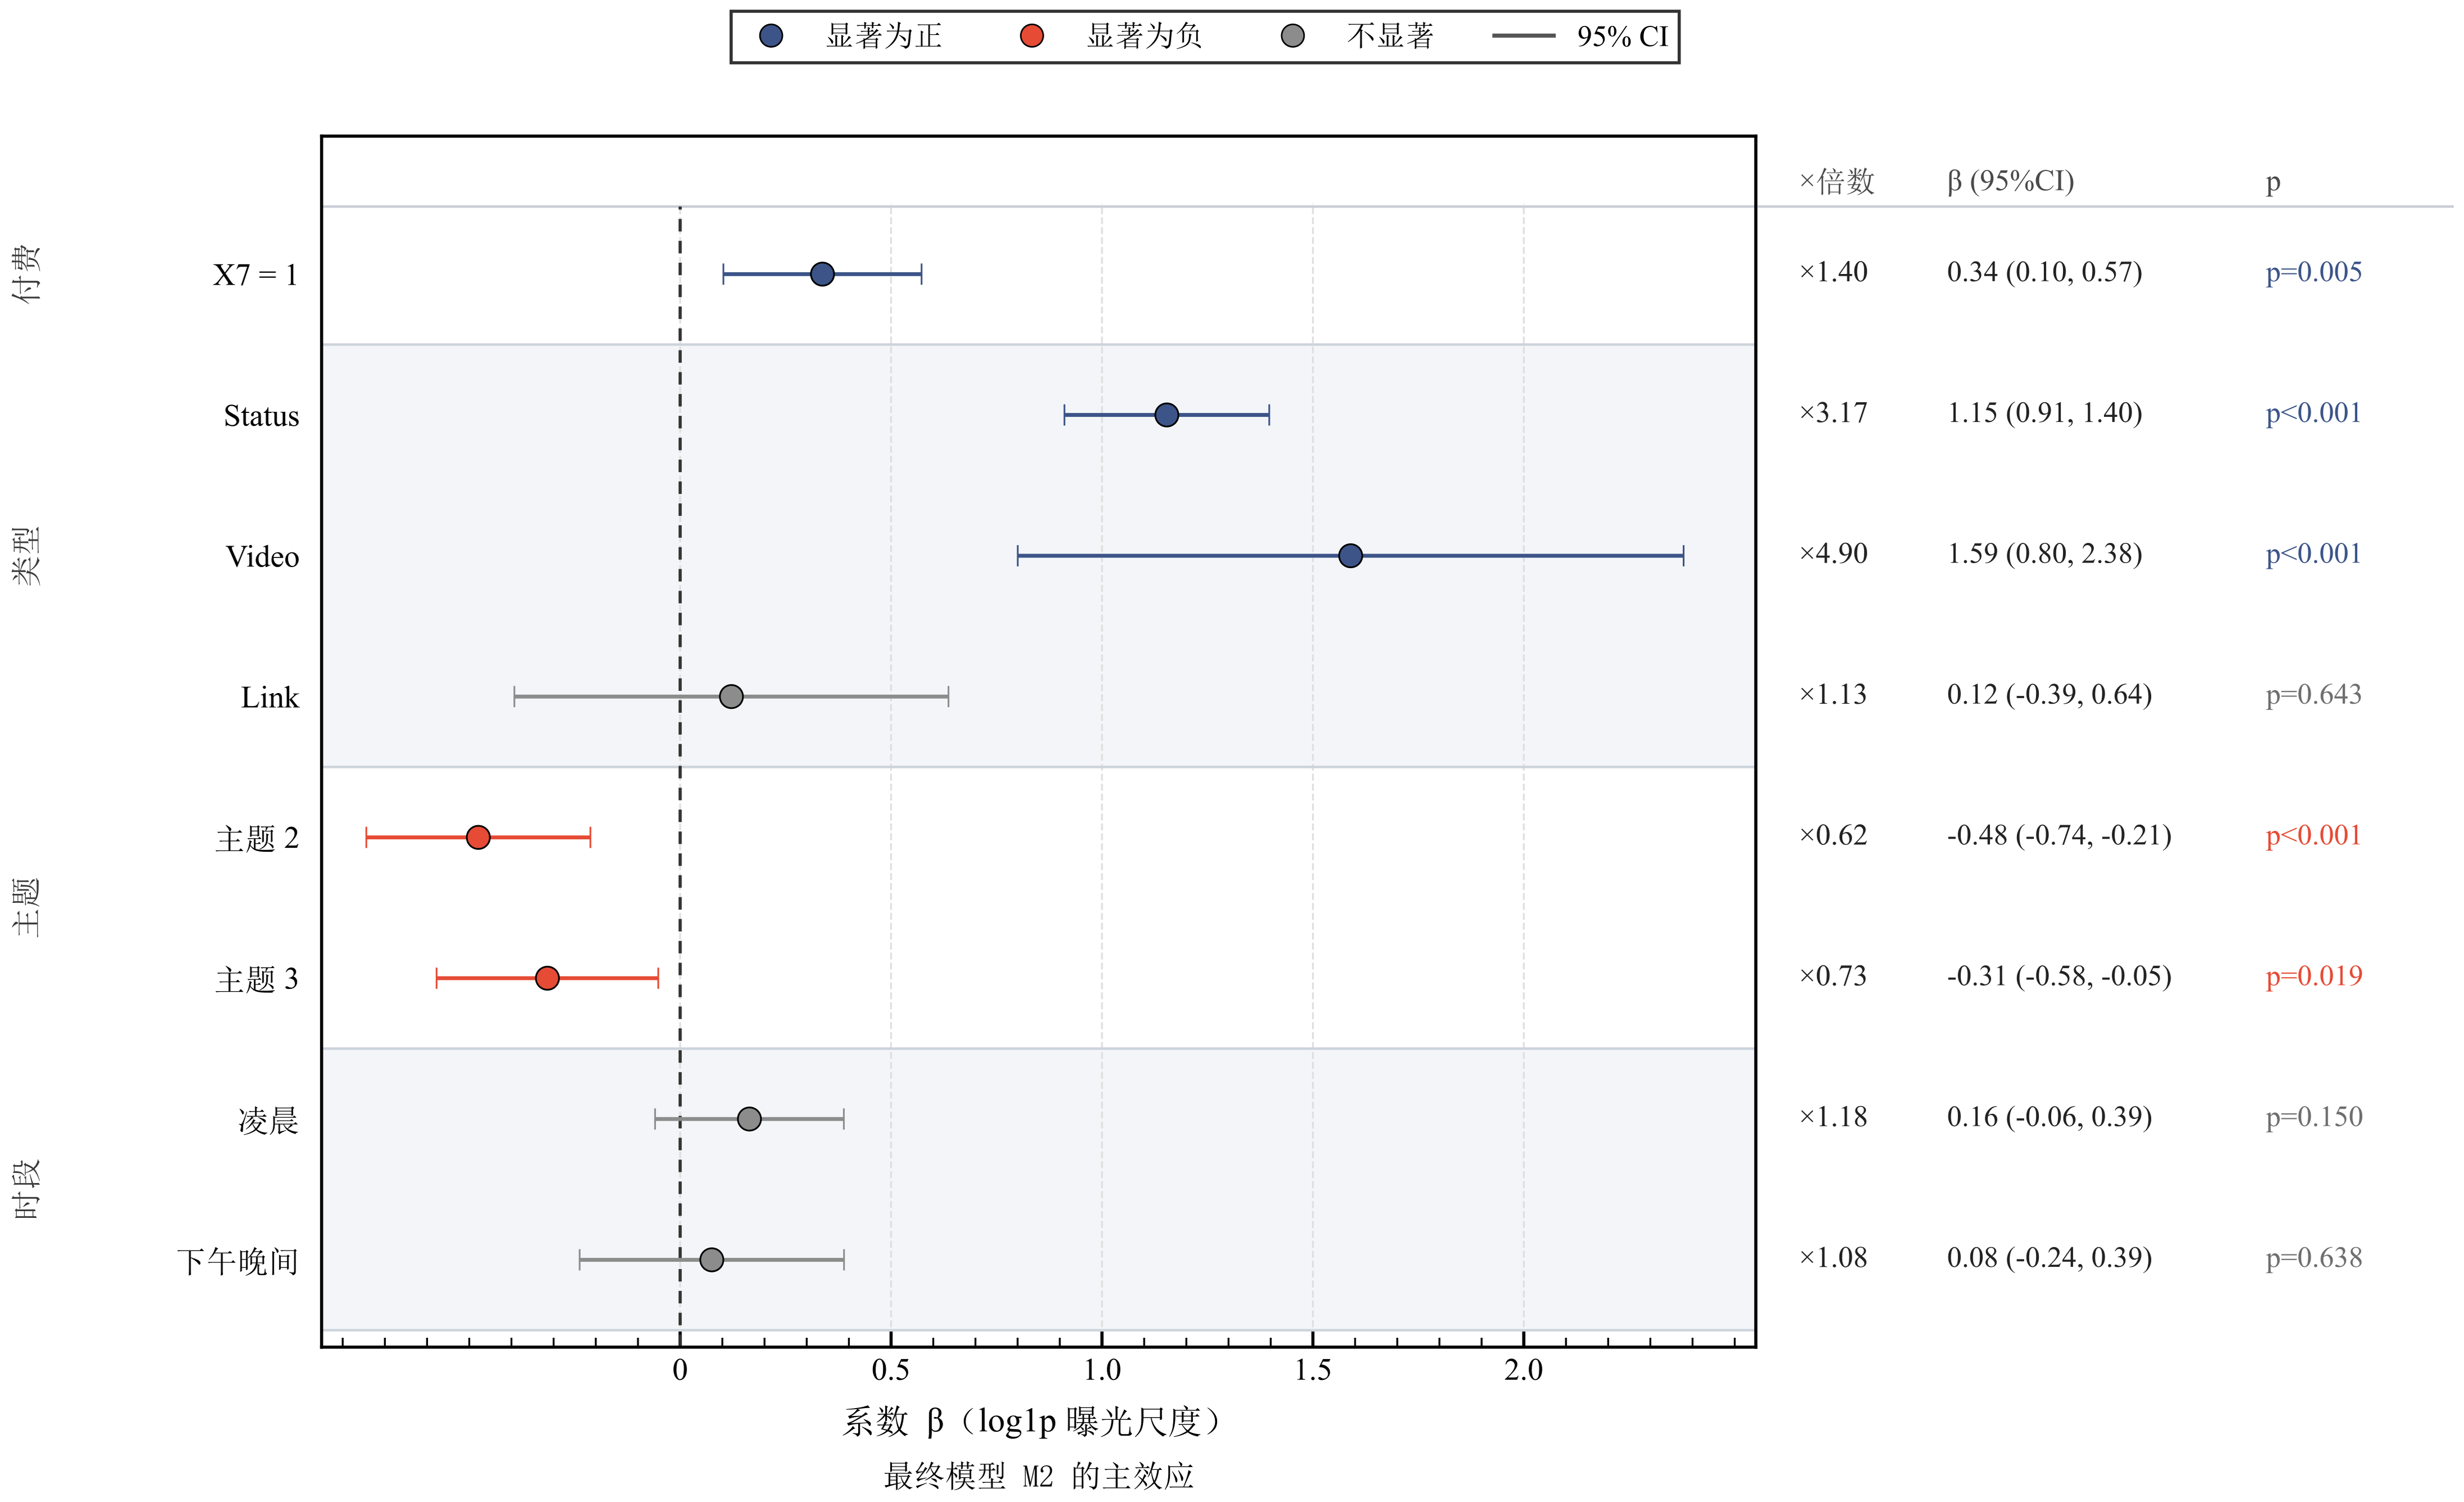
\includegraphics[width=0.76\textwidth]{../求解/问题三/结果/图6_最终模型系数森林图.png}
  \caption{最终模型的主效应系数与 95\% 置信区间}
  \label{fig:forest}
\end{figure}

\subsection{残差诊断与共线处理效果}

残差检验见表\ref{tab:resid}。Jarque--Bera 统计量 118.97、$p<0.001$，残差呈尖峰厚尾；Breusch--Pagan 统计量 56.52、$p=0.0005$，存在随拟合值增大的异方差；White 检验与 Ramsey RESET 同样拒绝同方差与线性形式正确的原假设。这三项结果共同决定了推断口径：系数显著性使用 HC3 稳健标准误，系数解释限定在样本内的局部平均效应。图\ref{fig:resid}给出四联诊断：残差对拟合值呈水平带状但离散度随拟合值扩大；标准化残差的 Q--Q 图两端偏离 45° 线；尺度—位置图显示绝对残差随拟合值上升；Cook 距离有 30 个观测超过 $4/n$ 阈值，最大的三条分别为第 416、141、461 号帖子，其影响力均在可接受范围内。

{\small
\begin{longtable}{>{\centering\arraybackslash}p{0.160\textwidth}>{\centering\arraybackslash}p{0.300\textwidth}>{\centering\arraybackslash}p{0.160\textwidth}>{\centering\arraybackslash}p{0.140\textwidth}>{\centering\arraybackslash}p{0.220\textwidth}}
  \caption{残差诊断检验结果}
  \label{tab:resid} \\
  \toprule
  模型 & 检验 & 统计量 & p值 & 判断 \\
  \midrule
  \endfirsthead
  \caption{残差诊断检验结果（续）} \\
  \toprule
  模型 & 检验 & 统计量 & p值 & 判断 \\
  \midrule
  \endhead
  \bottomrule
  \endfoot
  M1 全模型 & Jarque–Bera 正态性 & 119.0 & 0 & 残差非正态 \\
  M1 全模型 & Breusch–Pagan 异方差 & 56.5179 & 0.0005 & 存在异方差 \\
  M1 全模型 & White 异方差 & 283.3 & 0.0789 & 未检出/不可判定 \\
  M1 全模型 & Ramsey RESET（3 阶） & 2.867 & 0.0579 & 未检出设定误差 \\
  M1 全模型 & Durbin–Watson & 2.0513 & — & 接近 2，无强自相关（截面数据仅作参考） \\
  M1 全模型 & Cook 距离最大值 & 0.0492 & — & 无 Cook>1 的强影响点 \\
  M1 全模型 & 高杠杆点个数（h>2p/n） & 10 & — & 阈值 h>0.108 \\
  M2 最终模型 & Jarque–Bera 正态性 & 120.4 & 0 & 残差非正态 \\
  M2 最终模型 & Breusch–Pagan 异方差 & 54.7371 & 0.0005 & 存在异方差 \\
  M2 最终模型 & White 异方差 & 266.5 & 0.0301 & 存在异方差 \\
  M2 最终模型 & Ramsey RESET（3 阶） & 2.8451 & 0.0591 & 未检出设定误差 \\
  M2 最终模型 & Durbin–Watson & 2.0523 & — & 接近 2，无强自相关（截面数据仅作参考） \\
  M2 最终模型 & Cook 距离最大值 & 0.0377 & — & 无 Cook>1 的强影响点 \\
  M2 最终模型 & 高杠杆点个数（h>2p/n） & 10 & — & 阈值 h>0.104 \\
\end{longtable}
}


\begin{figure}[htbp]
  \centering
  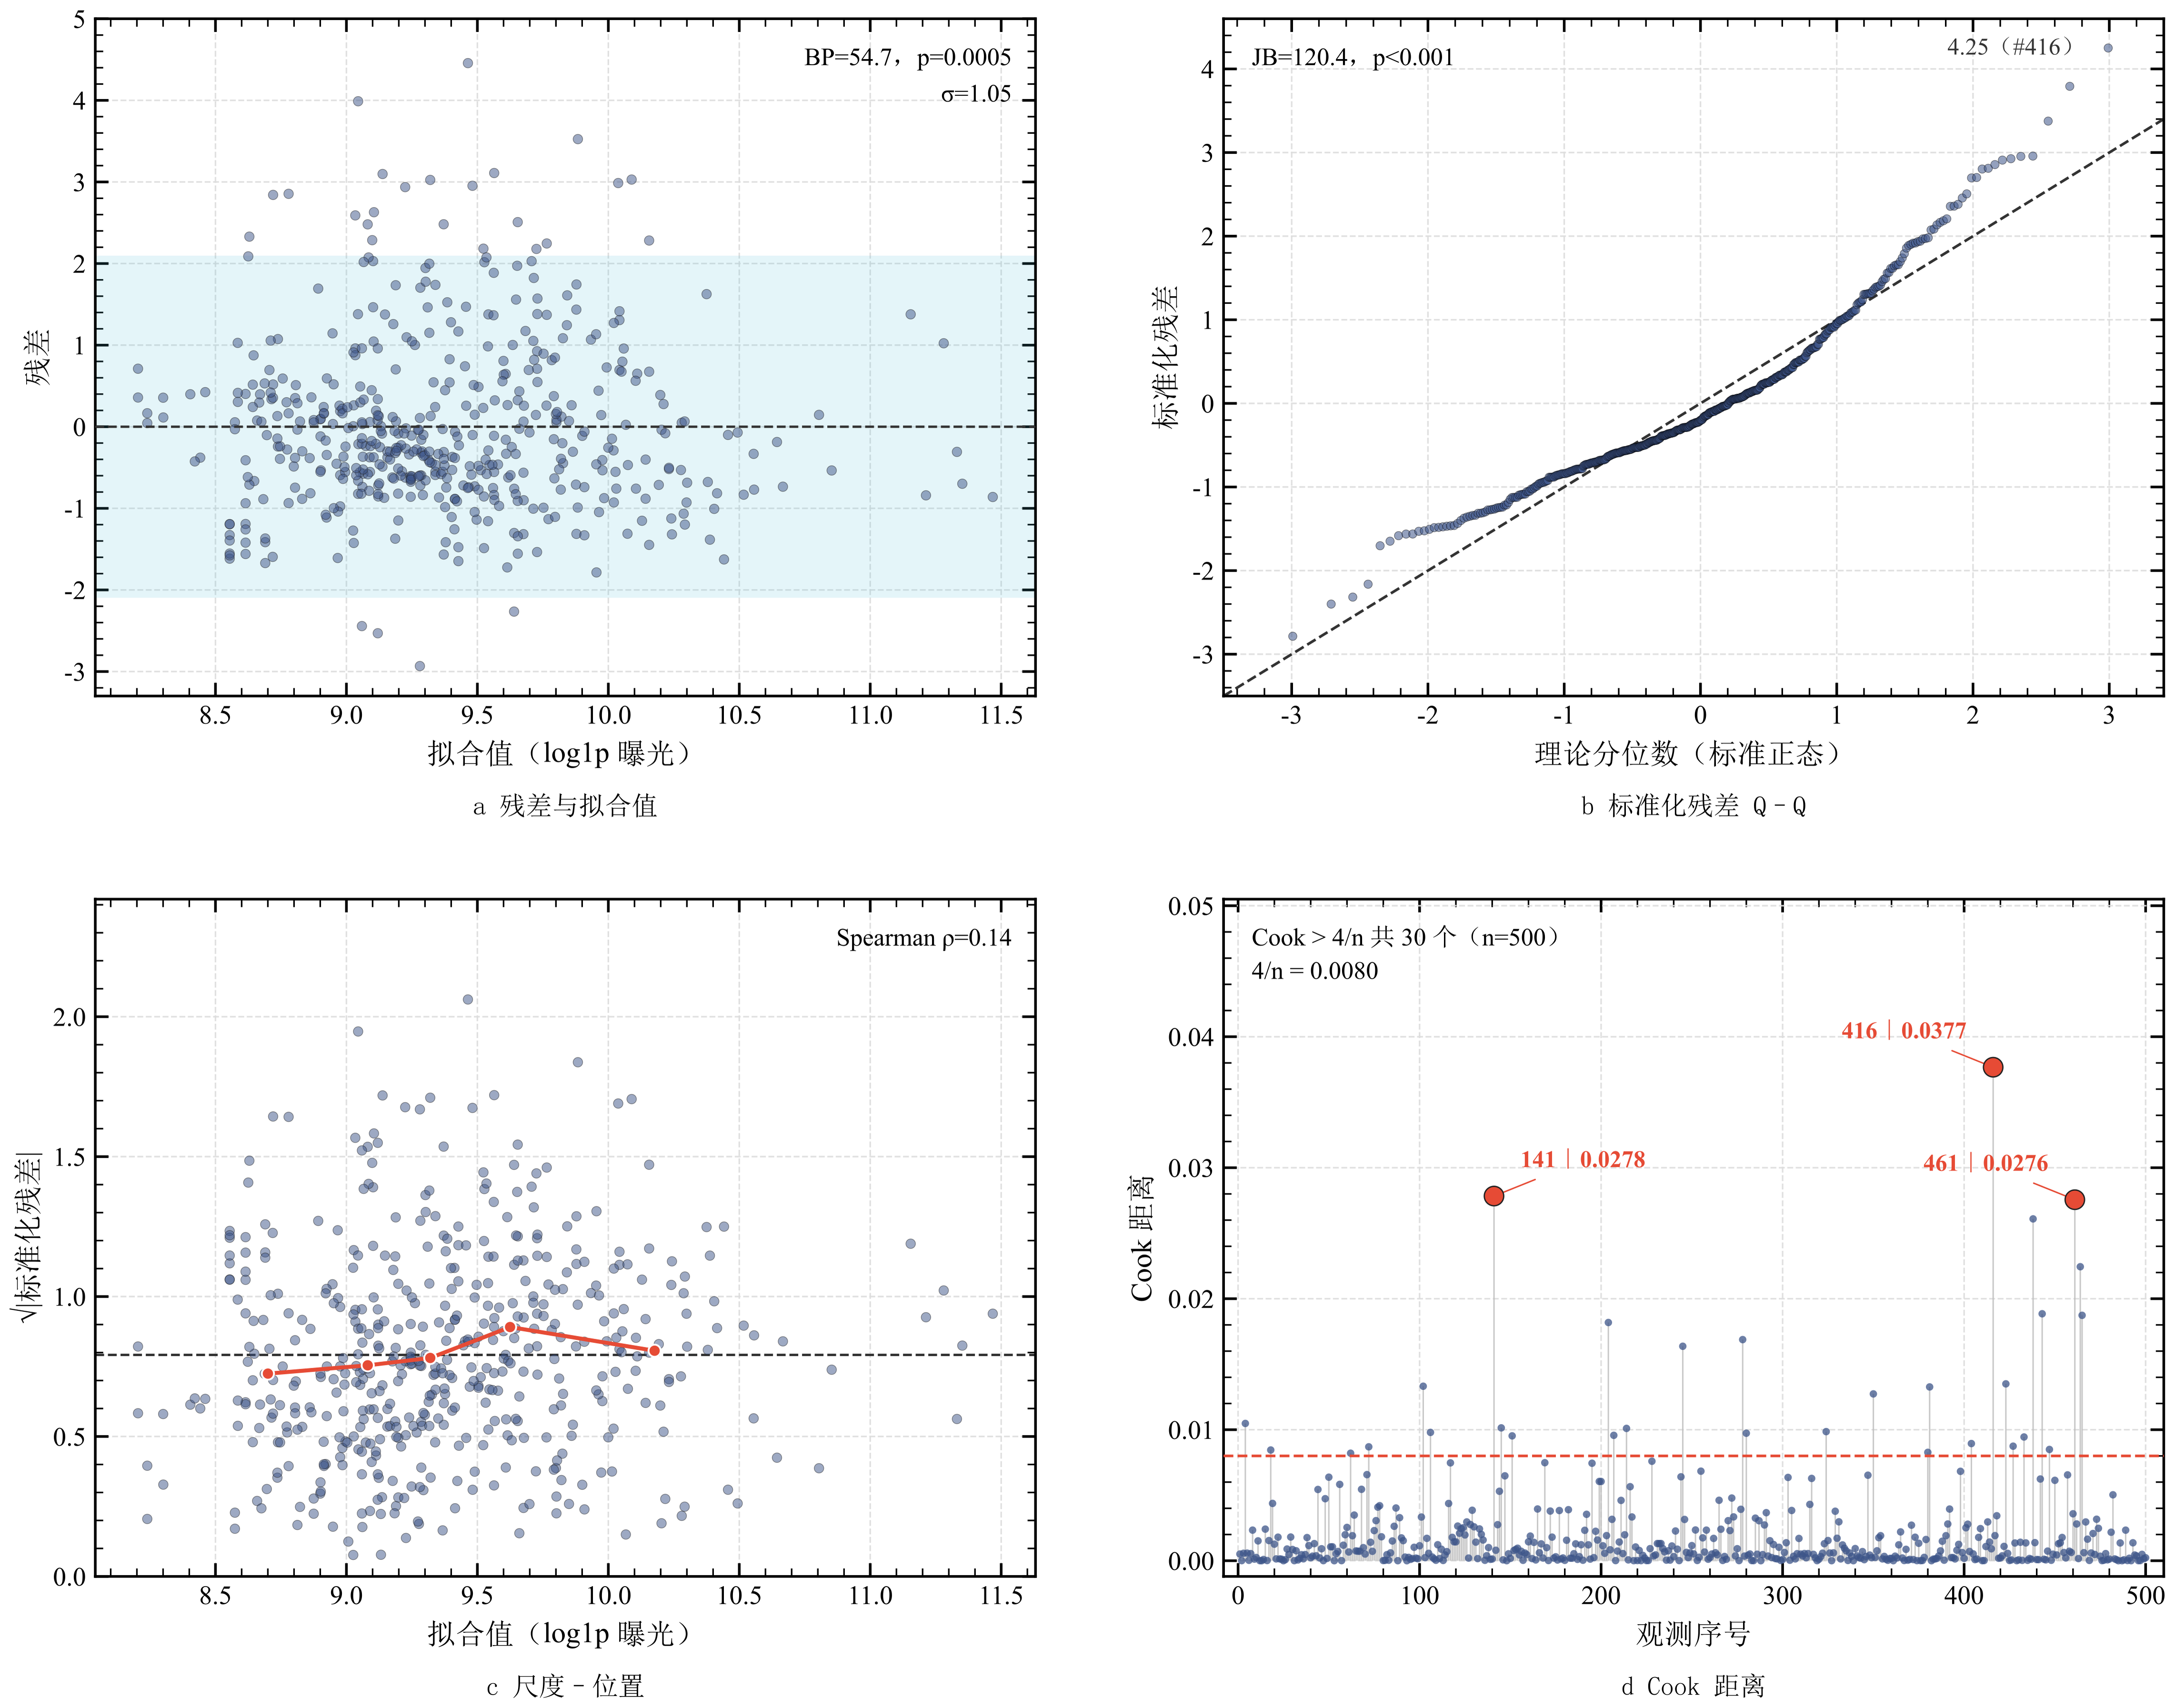
\includegraphics[width=0.65\textwidth]{../求解/问题三/结果/图8_残差诊断.png}
  \caption{最终模型的残差诊断：拟合、Q--Q、尺度—位置与 Cook 距离}
  \label{fig:resid}
\end{figure}

共线处理的直接效果见图\ref{fig:vif}。全模型 M1 中 $\log X_1$ 的方差膨胀因子为 124.9、月份哑变量组最大值为 143.0，远超 10 的严重共线阈值；剔除粉丝规模后，M2 的最大方差膨胀因子降至 3.23，全部解释变量落入可接受区间（$<5$）。哑铃图把每个变量的前后变化连在一起，除粉丝规模已不进入模型外，其余变量的方差膨胀因子几乎不变，说明共线只发生在粉丝规模与月份之间，与其他变量无关。

\begin{figure}[htbp]
  \centering
  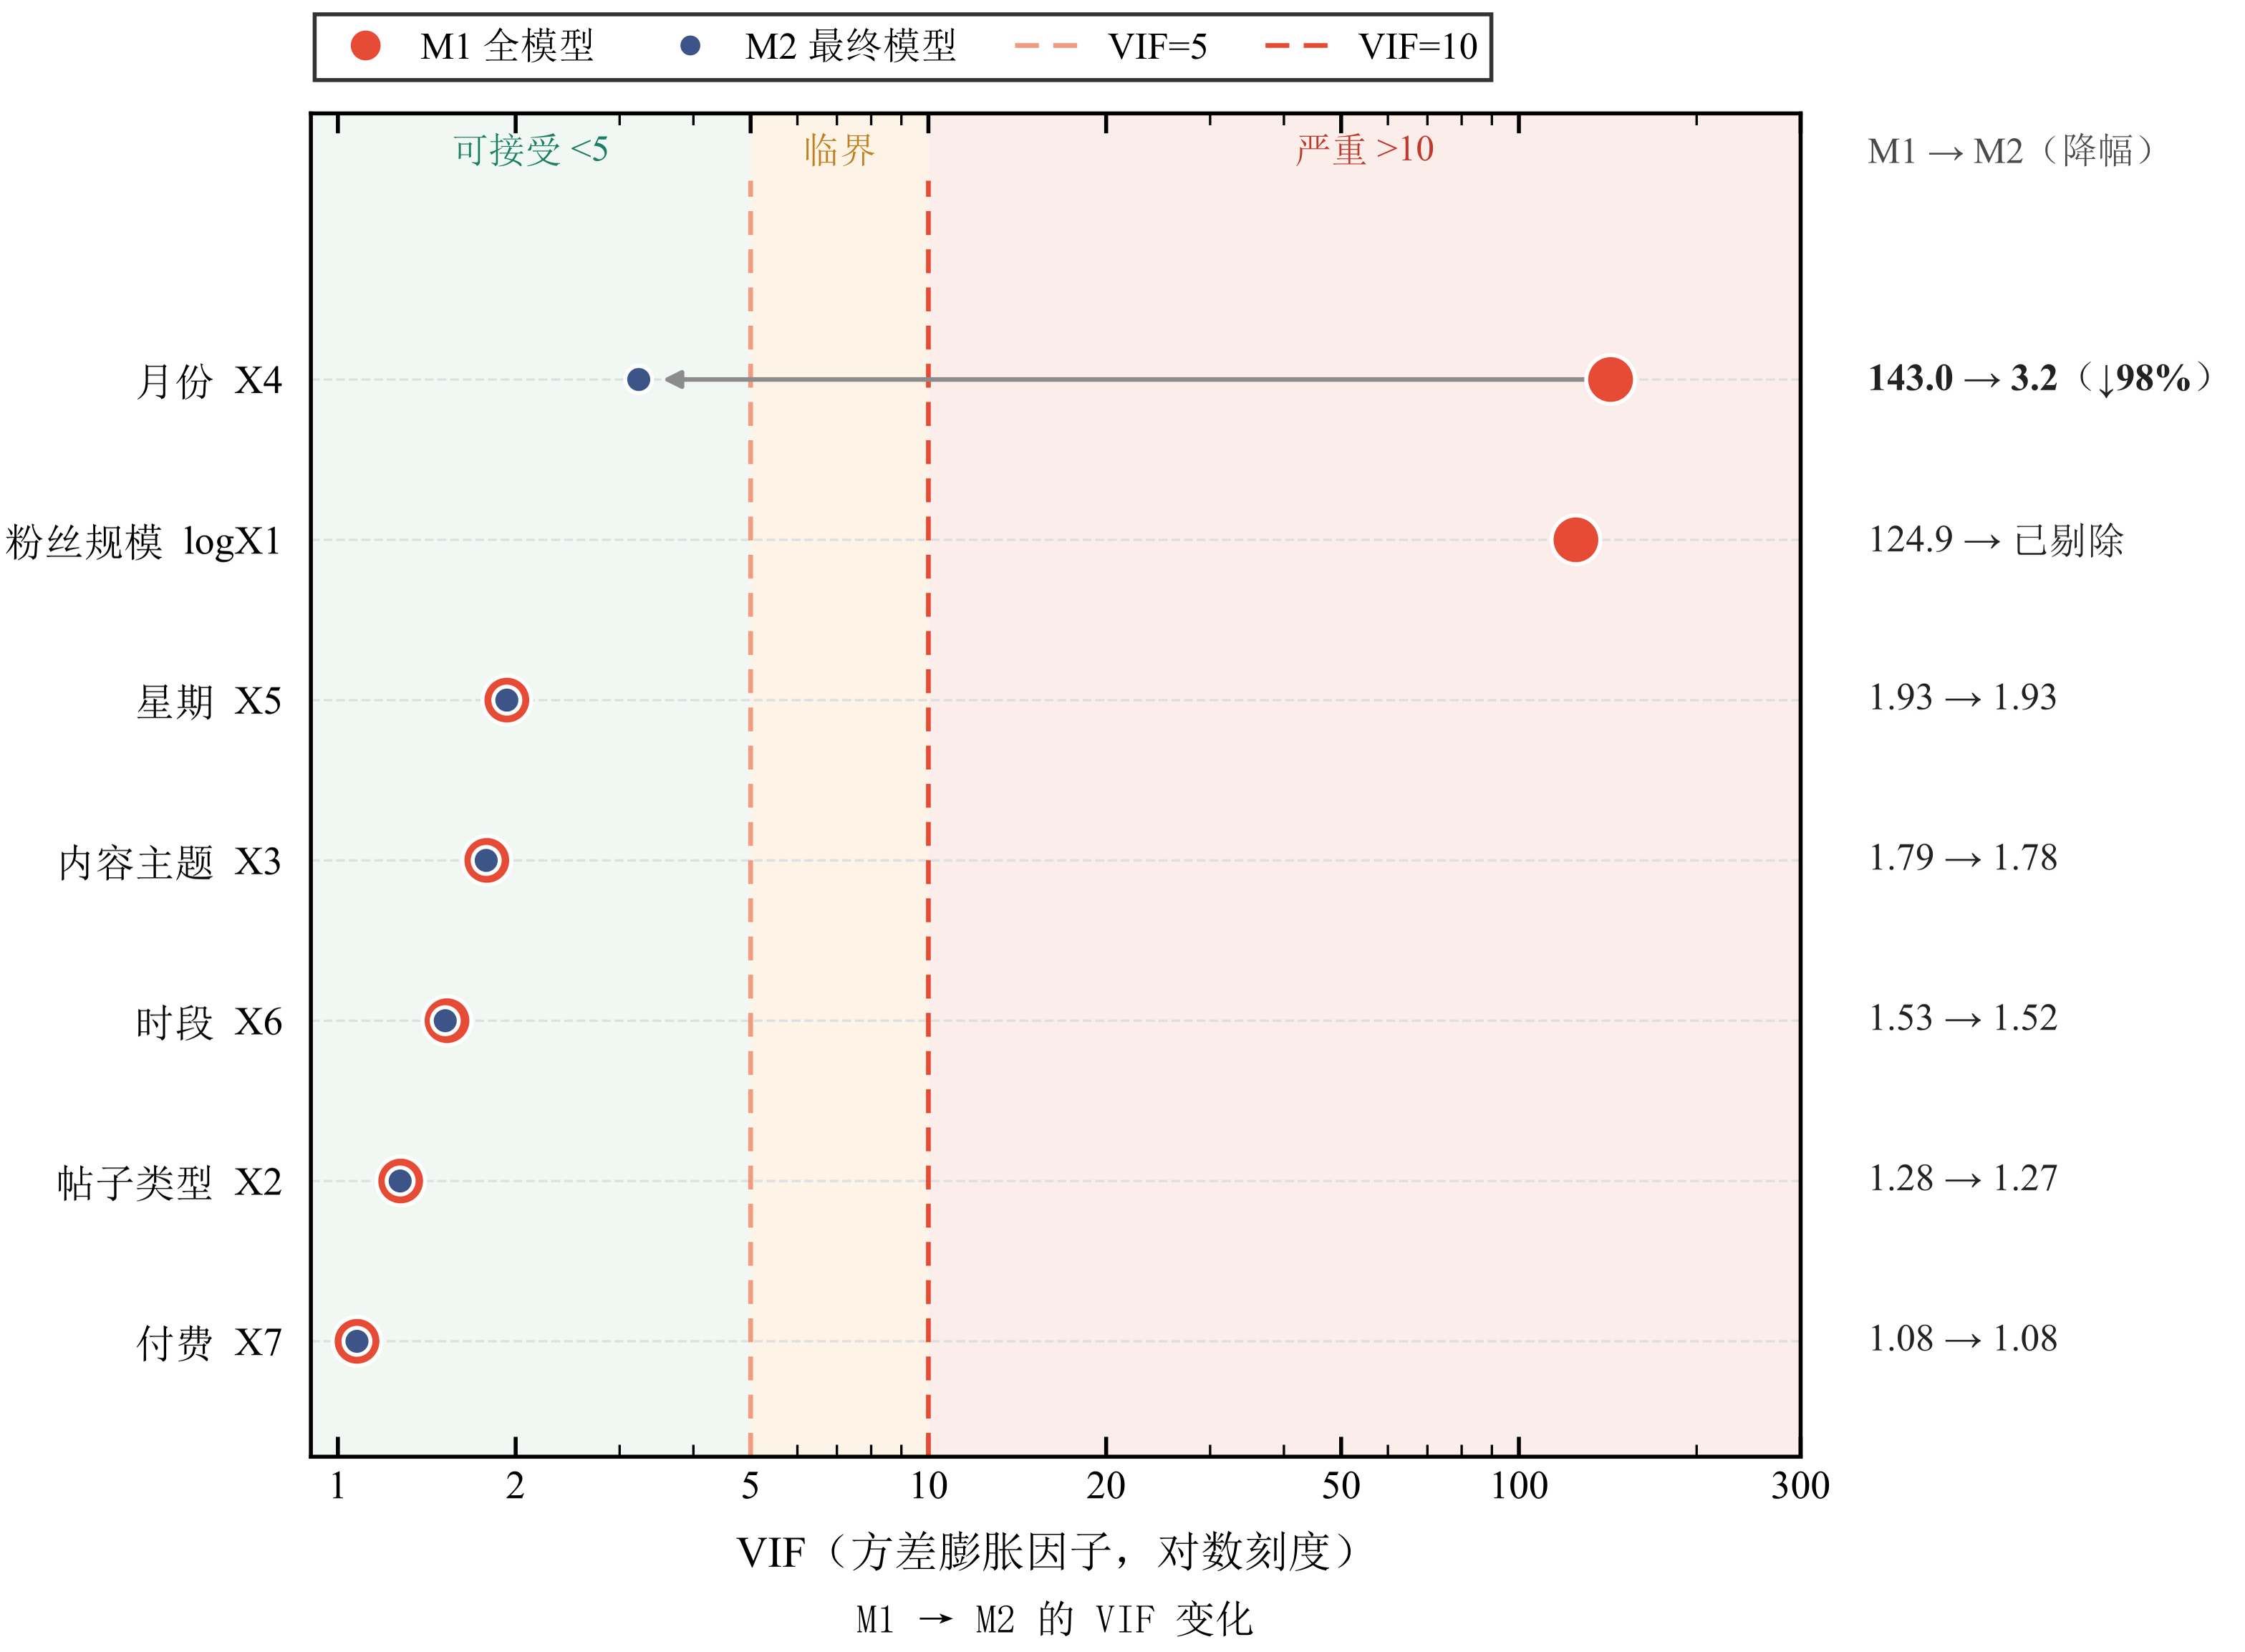
\includegraphics[width=0.65\textwidth]{../求解/问题三/结果/图7_共线性诊断.png}
  \caption{共线处理前后各方差膨胀因子的变化}
  \label{fig:vif}
\end{figure}

\subsection{预测能力}

图\ref{fig:cv}把五个候选的样本内 $R^2$ 与十折交叉验证 $R^2$ 用坡度图对照。所有模型都出现右倾——交叉验证表现低于样本内，这是参数估计用到全部样本的必然结果，但倾斜幅度不同：M1 从 0.207 降至 0.097，M2 从 0.207 降至 0.101，两者几乎重合；M3 与 M4 分别从 0.161 与 0.166 降至 0.094 与 0.097；M0 从 0 降至 $-0.021$。M2 的交叉验证 $R^2$ 最高、RMSE 最低，且比 M1 少一个参数，因此作为最终模型。样本外 $R^2$ 只有 0.10，说明模型适合判断变量方向与相对幅度，不适合逐条预测单帖曝光。

\begin{figure}[htbp]
  \centering
  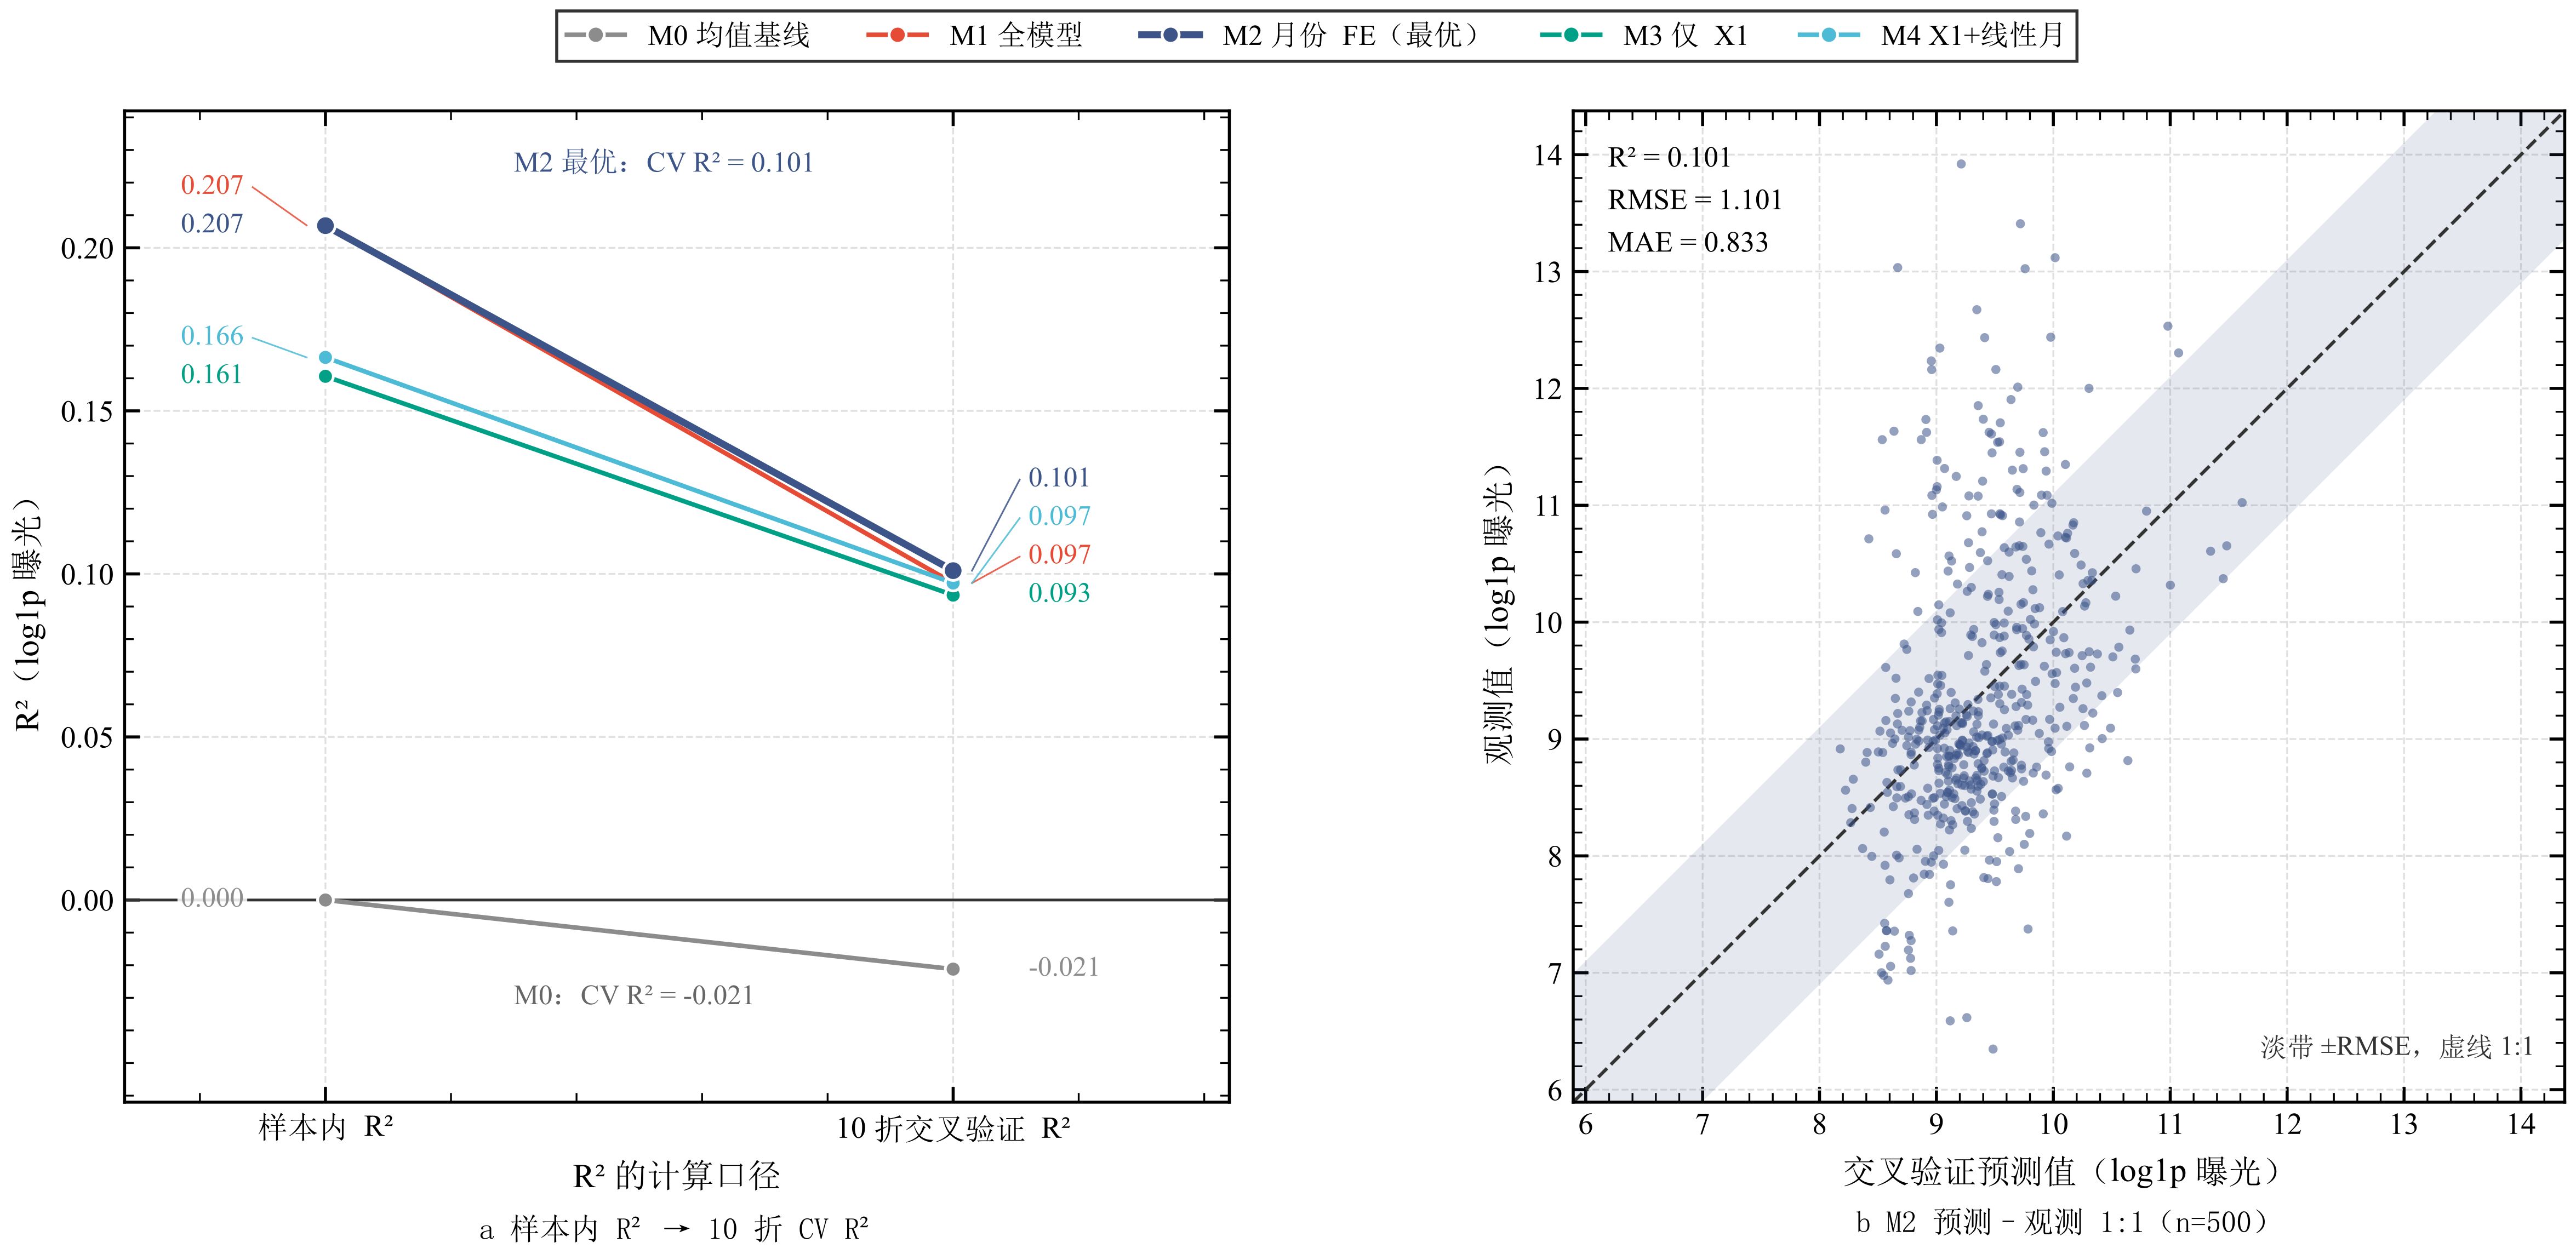
\includegraphics[width=0.76\textwidth]{../求解/问题三/结果/图9_预测能力验证.png}
  \caption{五个候选模型的样本内与交叉验证 $R^2$}
  \label{fig:cv}
\end{figure}

\subsection{方差贡献分解}

把七个变量组按 128 个子集做 Shapley 分解，结果见表\ref{tab:shap}：发帖类型贡献 0.0767（占可解释方差 37.1\%）、月份 0.0579（28.0\%）、付费 0.0244（11.8\%）、星期 0.0236（11.4\%）、内容主题 0.0142（6.9\%）、时段 0.0055（2.6\%）、粉丝规模 0.0046（2.2\%）。七个变量组合计解释 20.7\% 的曝光方差，剩余 79.3\% 属于个体差异与未观测因素。这一分解给出与回归系数一致的排序：发帖类型与月份是曝光差异的主要来源，付费与星期次之，粉丝规模在控制月份后几乎没有增量贡献。

{\small
\begin{longtable}{>{\centering\arraybackslash}p{0.240\textwidth}>{\centering\arraybackslash}p{0.120\textwidth}>{\centering\arraybackslash}p{0.200\textwidth}>{\centering\arraybackslash}p{0.220\textwidth}>{\centering\arraybackslash}p{0.200\textwidth}}
  \caption{七个变量组的 Shapley $R^2$ 分解}
  \label{tab:shap} \\
  \toprule
  变量组 & 自由度 & Shapley\_R² & 占已解释方差 & 占总方差 \\
  \midrule
  \endfirsthead
  \caption{七个变量组的 Shapley $R^2$ 分解（续）} \\
  \toprule
  变量组 & 自由度 & Shapley\_R² & 占已解释方差 & 占总方差 \\
  \midrule
  \endhead
  \bottomrule
  \endfoot
  发帖类型 X2 & 3 & 0.0767 & 0.3709 & 0.0767 \\
  内容主题 X3 & 2 & 0.0142 & 0.0688 & 0.0142 \\
  月份 X4 & 11 & 0.0579 & 0.2798 & 0.0579 \\
  星期 X5 & 6 & 0.0236 & 0.1142 & 0.0236 \\
  时段 X6 & 2 & 0.0055 & 0.0264 & 0.0055 \\
  付费 X7 & 1 & 0.0244 & 0.1179 & 0.0244 \\
  粉丝规模 logX1 & 1 & 0.0046 & 0.0220 & 0.0046 \\
  发帖决策合计（X2/X3/X5/X6/X7） & 13 & 0.1445 & 0.6982 & 0.1445 \\
  账号规模与时间合计（X1/X4） & 12 & 0.0624 & 0.3018 & 0.0624 \\
  未解释方差 & — & 0.7931 & — & 0.7931 \\
\end{longtable}
}


\subsection{效应测算}

系数的经济含义通过三个层次还原到曝光尺度。第一层用 $\exp(\beta)-1$ 给出百分比效应；第二层用 Duan 烟雾因子把对数尺度预测还原为曝光次数，在代表性画像（Photo、主题 1、7 月、周四、上午、粉丝 129,600）上计算反事实；第三层对 500 条帖子逐条反事实并取平均，得到样本平均处理效应。表\ref{tab:paid}给出付费效应的三层结果：系数 0.337 对应 40.1\% 的提升，代表性画像上自然帖子预期曝光 40,221 次、付费帖子 56,364 次，差值 16,142 次；全样本平均处理效应为 10,907 次。原始数据的中位数比（1.438）与模型结果（1.401）接近，说明调整前后结论稳定。

{\small
\begin{longtable}{>{\centering\arraybackslash}p{0.420\textwidth}>{\centering\arraybackslash}p{0.200\textwidth}>{\centering\arraybackslash}p{0.190\textwidth}>{\centering\arraybackslash}p{0.190\textwidth}}
  \caption{付费投放的曝光效应测算}
  \label{tab:paid} \\
  \toprule
  指标 & 估计值 & 95\%CI下限 & 95\%CI上限 \\
  \midrule
  \endfirsthead
  \caption{付费投放的曝光效应测算（续）} \\
  \toprule
  指标 & 估计值 & 95\%CI下限 & 95\%CI上限 \\
  \midrule
  \endhead
  \bottomrule
  \endfoot
  M2 付费系数 β & 0.3374 & 0.1025 & 0.5723 \\
  exp(β)−1（\%） & 40.1325 & 10.7962 & 77.2364 \\
  代表性画像：
自然帖子预测曝光 & 40,221 & 25,282 & 62,189 \\
  代表性画像：
付费帖子预测曝光 & 56,364 & 36,172 & 87,327 \\
  代表性画像：
差值（次） & 16,142 & 4,543 & 33,467 \\
  代表性画像：
倍数 & 1.4013 & 1.1036 & 1.753 \\
  全样本 ATE：
差值（次） & 10,907 & 3,138 & 20,195 \\
  全样本 ATE：
倍数 & 1.4013 & 1.1036 & 1.7531 \\
  原始数据：
付费组中位曝光 & 12,060 & — & — \\
  原始数据：
自然组中位曝光 & 8,387 & — & — \\
  原始数据：
中位数比 & 1.4379 & — & — \\
  原始数据：
均值比 & 1.4051 & — & — \\
\end{longtable}
}


表\ref{tab:type}与表\ref{tab:topic}给出内容类型与内容主题的效应。视频帖是图片帖的 4.90 倍（95\% 区间 2.23--10.79），Status 是 3.17 倍（2.49--4.04），Link 与 Photo 无显著差异；但视频帖仅 7 条，区间宽度是 Photo 组的 10 倍以上，只能作为方向性证据。主题的联合 Wald 检验 $p=0.0018$，主题 2 与主题 1 的差异显著（$p=0.0004$）、主题 3 与主题 1 的差异显著（$p=0.019$），主题 2 与主题 3 之间无显著差异。

{\small
\begin{longtable}{>{\centering\arraybackslash}p{0.180\textwidth}>{\centering\arraybackslash}p{0.140\textwidth}>{\centering\arraybackslash}p{0.120\textwidth}>{\centering\arraybackslash}p{0.140\textwidth}>{\centering\arraybackslash}p{0.180\textwidth}>{\centering\arraybackslash}p{0.180\textwidth}}
  \caption{内容类型相对 Photo 的曝光差异}
  \label{tab:type} \\
  \toprule
  对比 & 系数 & p值 & 倍数 & 倍数CI下限 & 倍数CI上限 \\
  \midrule
  \endfirsthead
  \caption{内容类型相对 Photo 的曝光差异（续）} \\
  \toprule
  对比 & 系数 & p值 & 倍数 & 倍数CI下限 & 倍数CI上限 \\
  \midrule
  \endhead
  \bottomrule
  \endfoot
  Video vs Photo & 1.5896 & 0.0001 & 4.9017 & 2.2262 & 10.7925 \\
  Status vs Photo & 1.1538 & 0 & 3.1702 & 2.4869 & 4.0412 \\
  Link vs Photo & 0.1215 & 0.6428 & 1.1292 & 0.6750 & 1.8891 \\
\end{longtable}
}


{\small
\begin{longtable}{>{\centering\arraybackslash}p{0.220\textwidth}>{\centering\arraybackslash}p{0.220\textwidth}>{\centering\arraybackslash}p{0.200\textwidth}>{\centering\arraybackslash}p{0.160\textwidth}>{\centering\arraybackslash}p{0.140\textwidth}}
  \caption{内容主题的联合检验与两两对比}
  \label{tab:topic} \\
  \toprule
  项目 & 对比 & 系数或统计量 & p值 & 倍数 \\
  \midrule
  \endfirsthead
  \caption{内容主题的联合检验与两两对比（续）} \\
  \toprule
  项目 & 对比 & 系数或统计量 & p值 & 倍数 \\
  \midrule
  \endhead
  \bottomrule
  \endfoot
  联合检验（Wald） & 主题2=主题3=0 & 12.6783 & 0.0018 & — \\
  主题2 vs 主题1 & 差异 & -0.4784 & 0.0004 & 0.6198 \\
  主题3 vs 主题1 & 差异 & -0.3147 & 0.0190 & 0.7300 \\
  主题2 vs 主题3 & 差异 & -0.1638 & 0.1864 & 0.8489 \\
\end{longtable}
}


\begin{figure}[htbp]
  \centering
  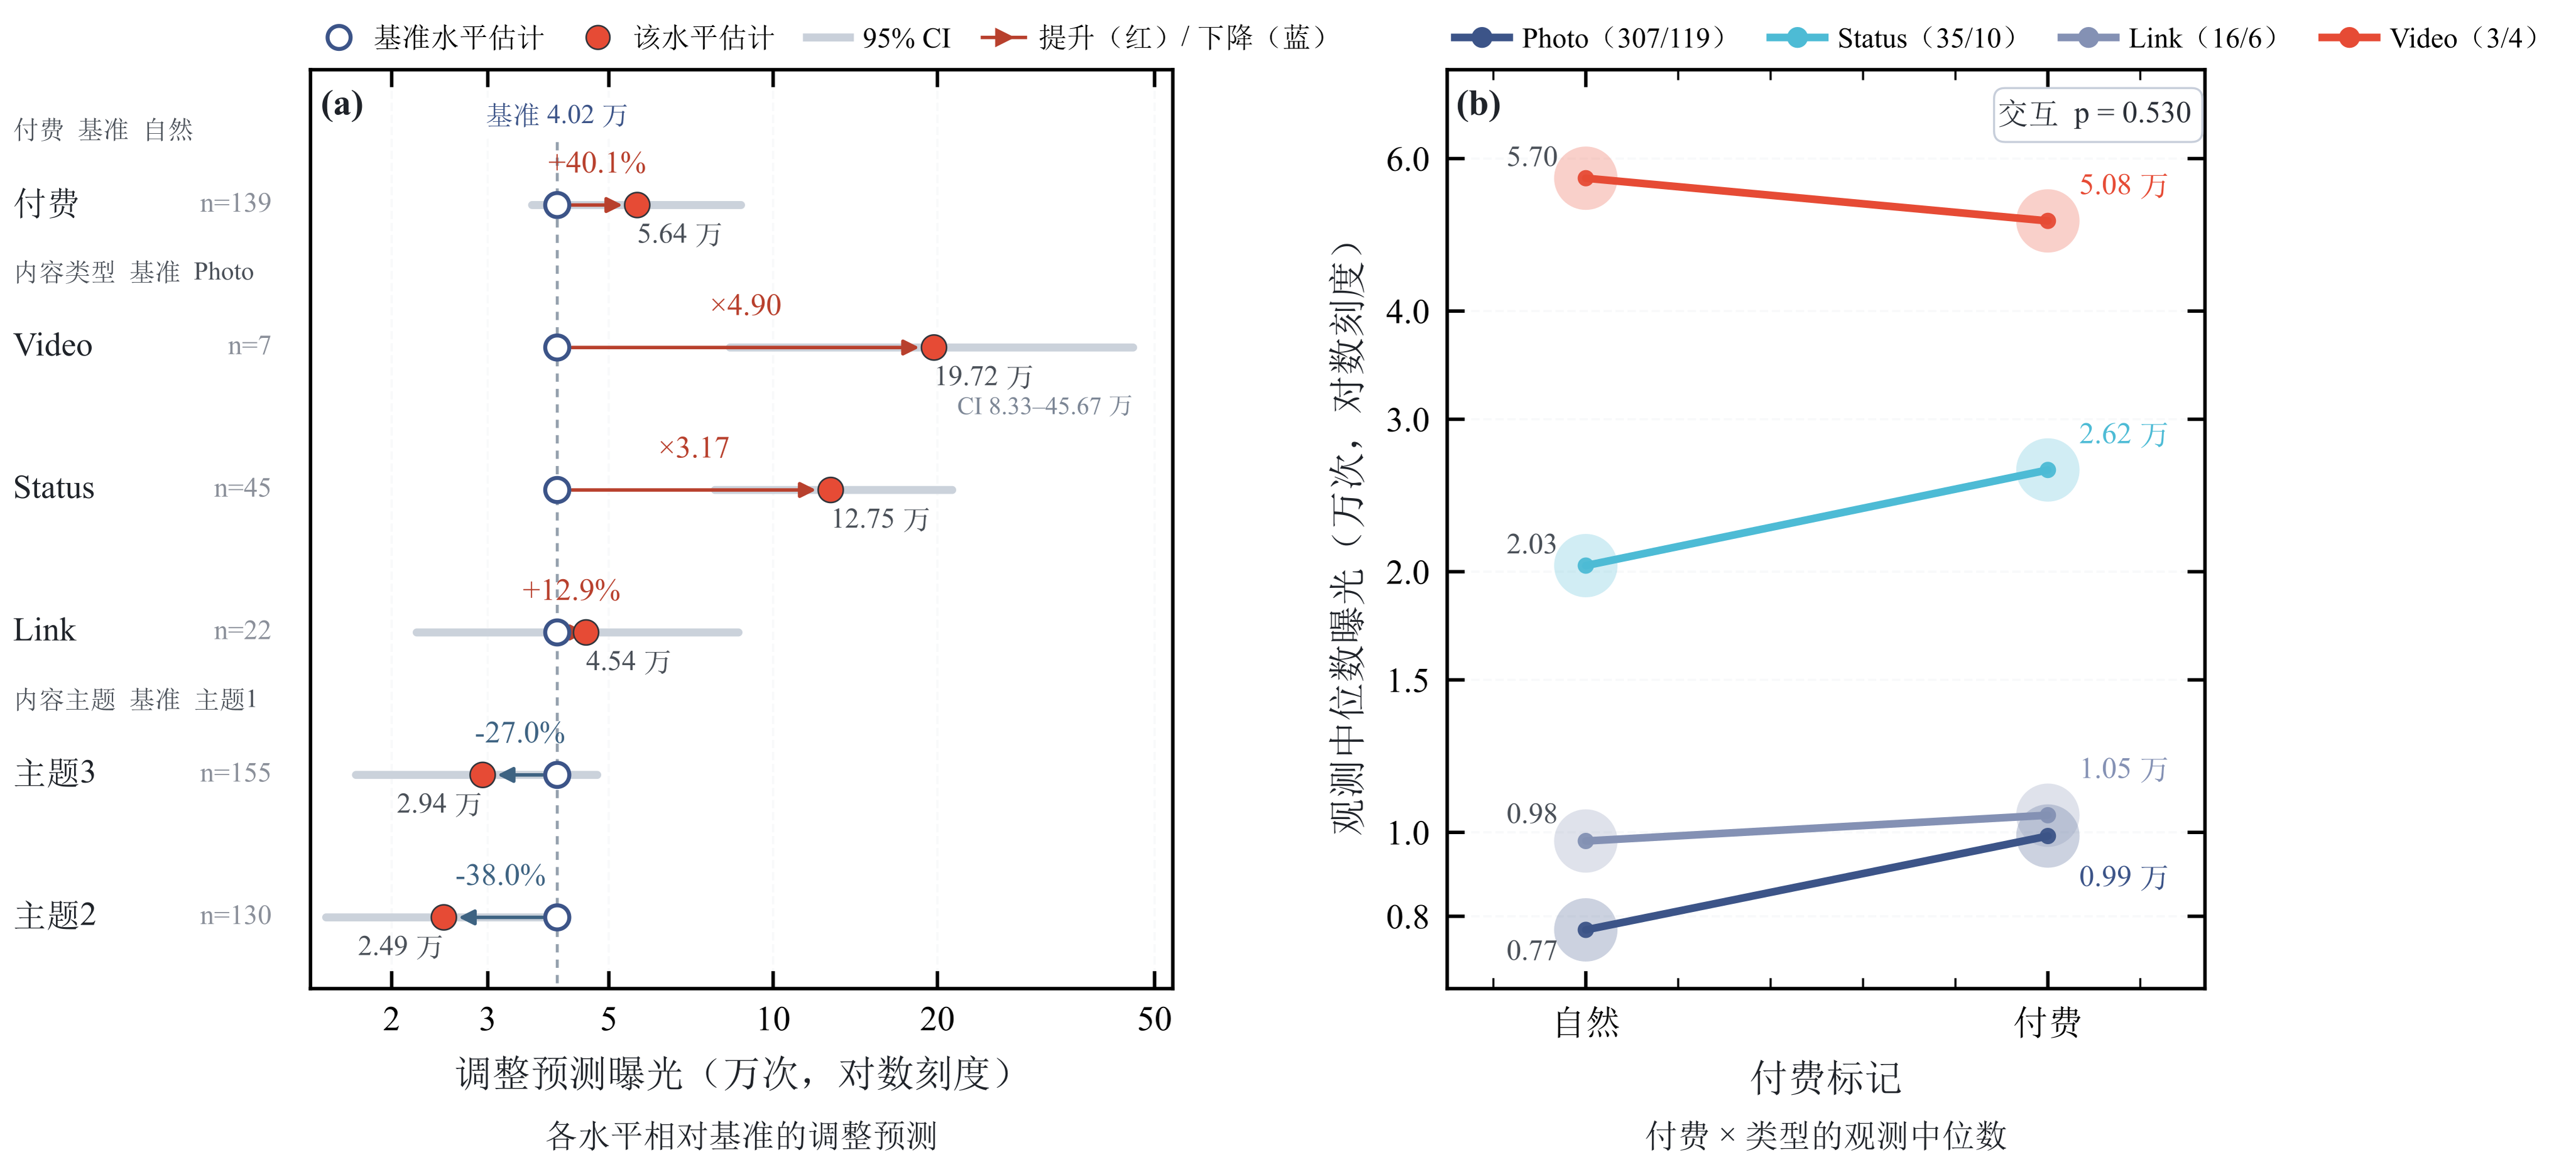
\includegraphics[width=0.76\textwidth]{../求解/问题四/结果/图11_调整预测效应.png}
  \caption{调整后的预测曝光：付费、内容类型与内容主题}
  \label{fig:adj}
\end{figure}

图\ref{fig:adj}把三组调整预测画在同一画布：付费组相对自然组提升 40.1\%，视频组 19.72 万次但区间最宽，主题 2 最低（2.49 万次）；右下图显示付费与类型的交互检验 $p=0.530$，交互项不显著，效应以主效应为主。

\subsection{稳健性与异质性}

六种模型设定下的效应见表\ref{tab:robust}与图\ref{fig:robust}。付费提升幅度在 37.4\%--49.6\% 之间，视频倍数在 3.52--5.41 之间，全部设定下方向一致、显著性不变；M3 与 M4 因剔除月份而略有上移，Huber 稳健回归与 Gamma GLM 给出更保守的估计，说明结论不依赖单一估计方法。

{\small
\begin{longtable}{>{\centering\arraybackslash}p{0.200\textwidth}>{\centering\arraybackslash}p{0.120\textwidth}>{\centering\arraybackslash}p{0.090\textwidth}>{\centering\arraybackslash}p{0.090\textwidth}>{\centering\arraybackslash}p{0.140\textwidth}>{\centering\arraybackslash}p{0.090\textwidth}>{\centering\arraybackslash}p{0.090\textwidth}>{\centering\arraybackslash}p{0.120\textwidth}}
  \caption{六种模型设定下的效应稳健性}
  \label{tab:robust} \\
  \toprule
  设定 & 付费提升（\%） & 提升下限 & 提升上限 & Video 倍数 & 倍数下限 & 倍数上限 & $X_3$ 联合 $p$ \\
  \midrule
  \endfirsthead
  \caption{六种模型设定下的效应稳健性（续）} \\
  \toprule
  设定 & 付费提升（\%） & 提升下限 & 提升上限 & Video 倍数 & 倍数下限 & 倍数上限 & $X_3$ 联合 $p$ \\
  \midrule
  \endhead
  \bottomrule
  \endfoot
  M1 全模型 & 40.0891 & 10.7199 & 77.2487 & 4.8944 & 2.2284 & 10.7499 & 0.0019 \\
  M2 月份固定效应 & 40.1325 & 10.8626 & 77.1301 & 4.9017 & 2.2307 & 10.7708 & 0.0018 \\
  M3 仅logX1 & 49.6482 & 18.5385 & 88.9225 & 5.2503 & 2.5022 & 11.0164 & 0.0052 \\
  M4 logX1+线性月份 & 47.137 & 15.8511 & 86.8717 & 5.4076 & 2.6179 & 11.17 & 0.0030 \\
  Huber 稳健回归 & 37.4423 & 13.2266 & 66.837 & 5.3838 & 2.5841 & 11.2168 & 0.0045 \\
  Gamma GLM（log 链接） & 44.8408 & 9.4426 & 91.6882 & 3.518 & 1.7216 & 7.1886 & 0.0001 \\
\end{longtable}
}


\begin{figure}[htbp]
  \centering
  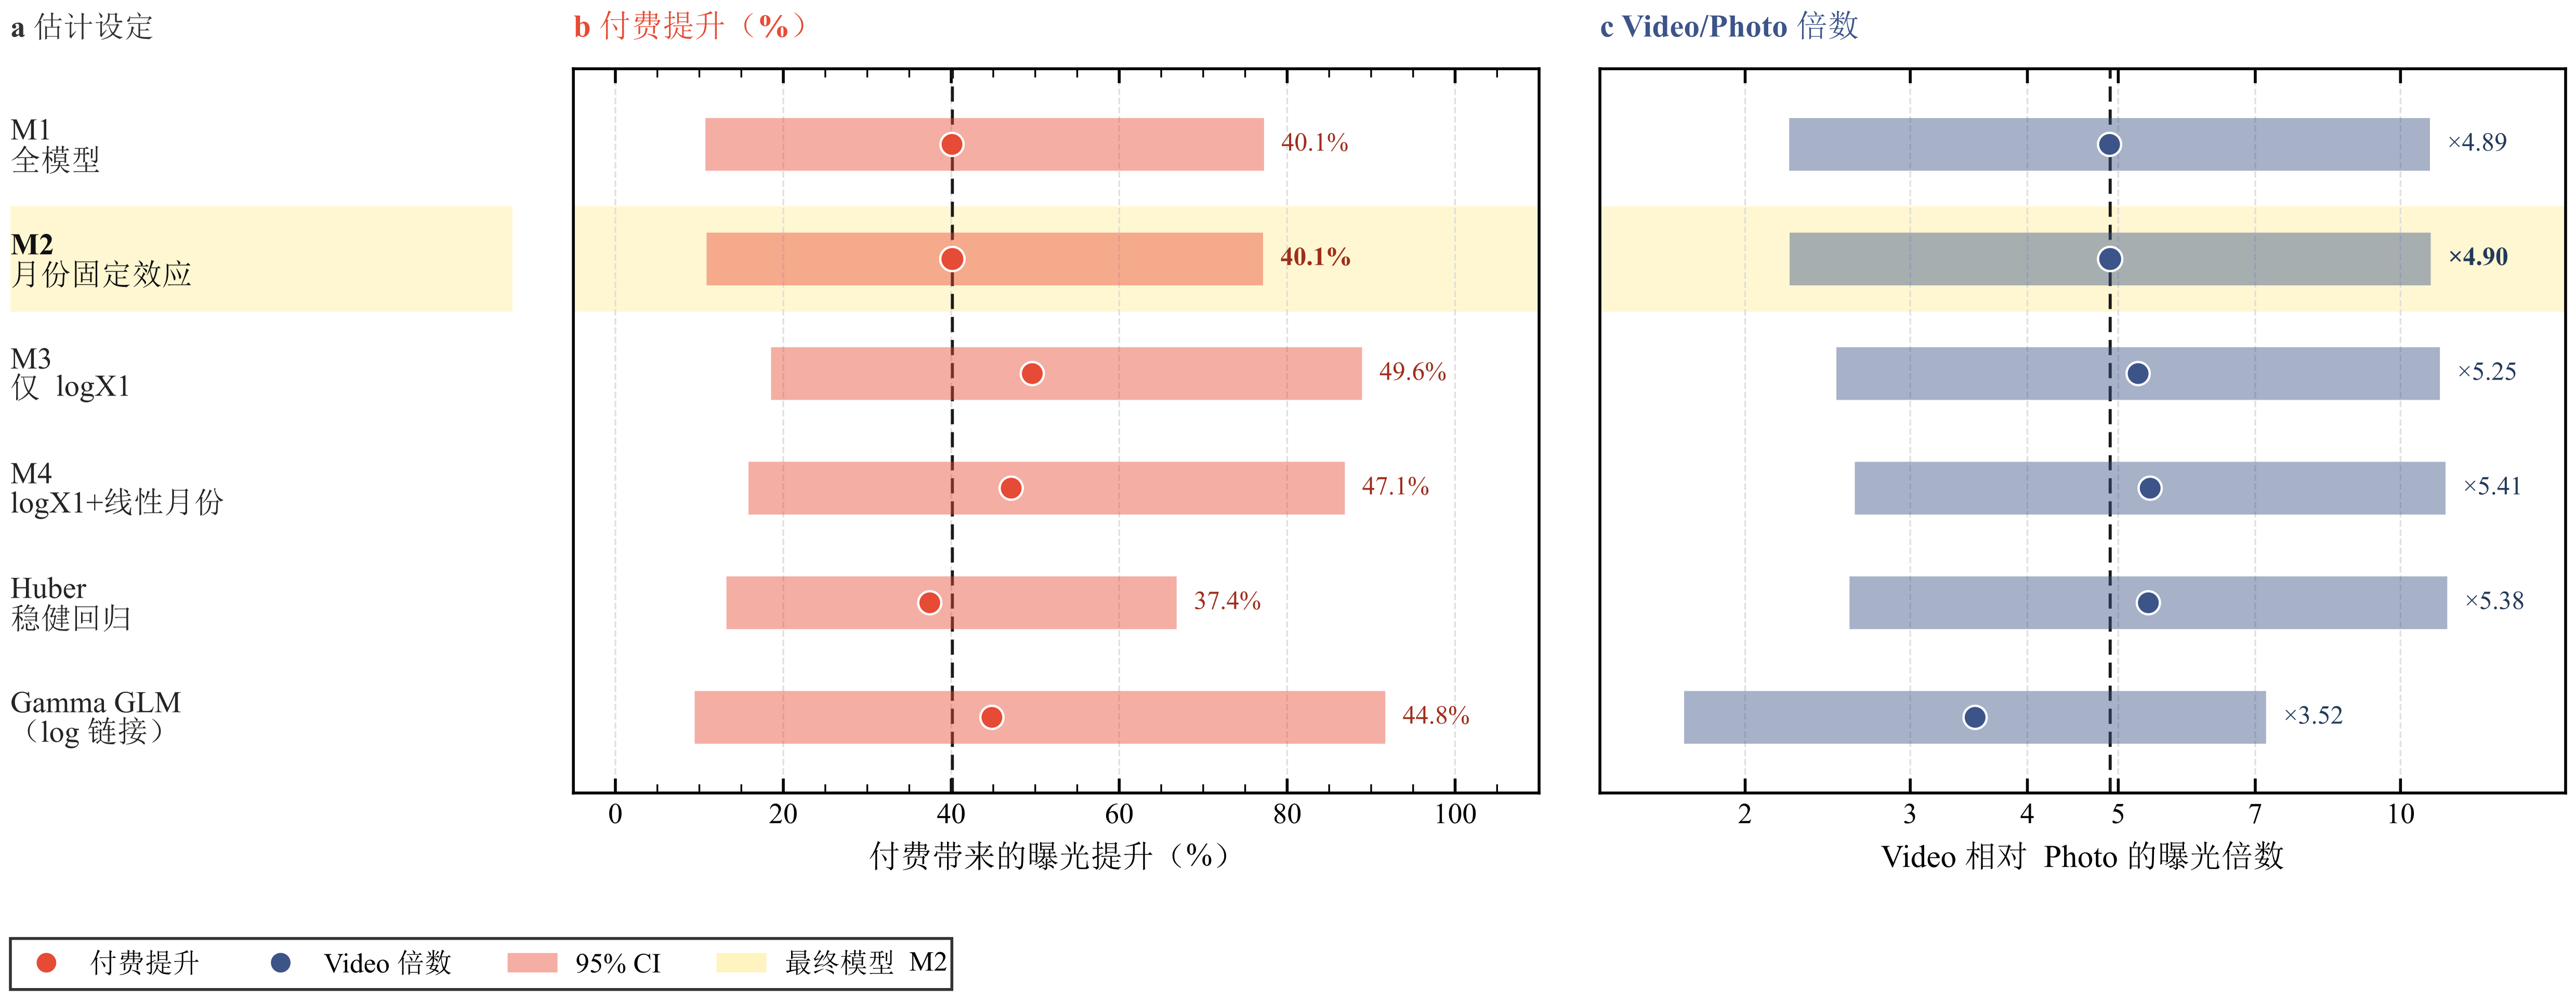
\includegraphics[width=0.77\textwidth]{../求解/问题四/结果/图12_效应稳健性.png}
  \caption{六种设定下的付费提升幅度与视频曝光倍数}
  \label{fig:robust}
\end{figure}

按子样本重估同一规格模型，结果见表\ref{tab:hetero}。类型与时段内部的付费效应没有显著差异（组内 $p=0.531$、$p=0.474$），但内容主题内部存在异质性（组内 $p=0.036$）：主题 1 的付费系数为 0.571（$p=0.008$），主题 3 仅为 0.018（$p=0.911$）。这意味着“付费提升四成”这一平均效应主要由主题 1 的帖子贡献，主题 3 的帖子几乎无法通过付费获得额外曝光。视频（7 条）与链接（22 条）子样本的自由度过低，其系数只能标注为参考，不能用于决策。

{\small
\begin{longtable}{>{\centering\arraybackslash}p{0.150\textwidth}>{\centering\arraybackslash}p{0.160\textwidth}>{\centering\arraybackslash}p{0.090\textwidth}>{\centering\arraybackslash}p{0.140\textwidth}>{\centering\arraybackslash}p{0.130\textwidth}>{\centering\arraybackslash}p{0.130\textwidth}>{\centering\arraybackslash}p{0.120\textwidth}}
  \caption{付费效应的子样本异质性}
  \label{tab:hetero} \\
  \toprule
  分组 & 子样本 & $N$ & 系数 & 下限 & 上限 & $p$ \\
  \midrule
  \endfirsthead
  \caption{付费效应的子样本异质性（续）} \\
  \toprule
  分组 & 子样本 & $N$ & 系数 & 下限 & 上限 & $p$ \\
  \midrule
  \endhead
  \bottomrule
  \endfoot
  全样本 & 全样本 & 500 & 0.3374 & 0.1025 & 0.5723 & 0.0050 \\
  帖子类型 & Photo & 426 & 0.3891 & 0.1289 & 0.6492 & 0.0035 \\
  帖子类型 & Status & 45 & 0.3526 & -0.2869 & 0.9921 & 0.2669 \\
  帖子类型 & Link & 22 & -0.5491 & -2.9451 & 1.8469 & 0.6207 \\
  帖子类型 & Video & 7 & -0.1900 & -2.6262 & 2.2463 & 0.8490 \\
  内容主题 & 主题 1 & 215 & 0.5700 & 0.1528 & 0.9872 & 0.0077 \\
  内容主题 & 主题 2 & 130 & 0.4251 & -0.0114 & 0.8616 & 0.0562 \\
  内容主题 & 主题 3 & 155 & 0.0239 & -0.3985 & 0.4462 & 0.9112 \\
  发布时段 & 凌晨 & 196 & 0.5937 & 0.2166 & 0.9708 & 0.0022 \\
  发布时段 & 上午 & 193 & 0.2368 & -0.1538 & 0.6274 & 0.2330 \\
  发布时段 & 下午晚间 & 111 & 0.2022 & -0.3237 & 0.7282 & 0.4470 \\
\end{longtable}
}

